
%(BEGIN_QUESTION)
% Copyright 2010, Tony R. Kuphaldt, released under the Creative Commons Attribution License (v 1.0)
% This means you may do almost anything with this work of mine, so long as you give me proper credit

Suppose the lamp refuses to light up when the pushbutton switch is pressed.  A voltmeter registers 12 volts between test points {\bf C} and {\bf E} in the circuit while the pushbutton is released (not pressed):

$$\includegraphics[width=15.5cm]{i04653x01.eps}$$

Identify the likelihood of each specified fault for this circuit.  Consider each fault one at a time (i.e. no coincidental faults), determining whether or not each fault could independently account for {\it all} measurements and symptoms in this circuit.

% No blank lines allowed between lines of an \halign structure!
% I use comments (%) instead, so that TeX doesn't choke.

$$\vbox{\offinterlineskip
\halign{\strut
\vrule \quad\hfil # \ \hfil & 
\vrule \quad\hfil # \ \hfil & 
\vrule \quad\hfil # \ \hfil \vrule \cr
\noalign{\hrule}
%
% First row
{\bf Fault} & {\bf Possible} & {\bf Impossible} \cr
%
\noalign{\hrule}
%
% Another row
Open wire between A and C &  &  \cr
%
\noalign{\hrule}
%
% Another row
Open wire between B and D &  &  \cr
%
\noalign{\hrule}
%
% Another row
Open wire between D and F &  &  \cr
%
\noalign{\hrule}
%
% Another row
Lamp failed open &  &  \cr
%
\noalign{\hrule}
%
% Another row
Switch failed open &  &  \cr
%
\noalign{\hrule}
%
% Another row
Lamp failed shorted &  &  \cr
%
\noalign{\hrule}
%
% Another row
Switch failed shorted &  &  \cr
%
\noalign{\hrule}
%
% Another row
Voltage source dead &  &  \cr
%
\noalign{\hrule}
} % End of \halign 
}$$ % End of \vbox

Finally, identify the {\it next} diagnostic test or measurement you would make on this system.  Explain how the result(s) of this next test or measurement help further identify the location and/or nature of the fault.

\vfil 

\underbar{file i04653}
\eject
%(END_QUESTION)





%(BEGIN_ANSWER)

% No blank lines allowed between lines of an \halign structure!
% I use comments (%) instead, so that TeX doesn't choke.

$$\vbox{\offinterlineskip
\halign{\strut
\vrule \quad\hfil # \ \hfil & 
\vrule \quad\hfil # \ \hfil & 
\vrule \quad\hfil # \ \hfil \vrule \cr
\noalign{\hrule}
%
% First row
{\bf Fault} & {\bf Possible} & {\bf Impossible} \cr
%
\noalign{\hrule}
%
% Another row
Open wire between A and C &  & $\surd$ \cr
%
\noalign{\hrule}
%
% Another row
Open wire between B and D &  & $\surd$ \cr
%
\noalign{\hrule}
%
% Another row
Open wire between D and F &  & $\surd$ \cr
%
\noalign{\hrule}
%
% Another row
Lamp failed open &  & $\surd$ \cr
%
\noalign{\hrule}
%
% Another row
Switch failed open & $\surd$ &  \cr
%
\noalign{\hrule}
%
% Another row
Lamp failed shorted & $\surd$ &  \cr
%
\noalign{\hrule}
%
% Another row
Switch failed shorted &  & $\surd$ \cr
%
\noalign{\hrule}
%
% Another row
Voltage source dead &  & $\surd$ \cr
%
\noalign{\hrule}
} % End of \halign 
}$$ % End of \vbox


%(END_ANSWER)





%(BEGIN_NOTES)


%INDEX% Troubleshooting review: electric circuits

%(END_NOTES)

